\newcommand{\scriptusage}{\\Run \texttt{Rscript main.R --help} for more details
on script usage.}

\chapter{Project part 2}\label{chp:part2}
\section{Tasks}
\begin{enumerate}
\setcounter{enumi}{8}

\item Implement in the language of your choice a program to create a wig file
with physical covarage. An example can be found in \filef{physical.pl}, but it
would be nice to implement the suggestions described in 
\filef{physical\_coverage.pdf}.
\label{itm:2.9}

\item Create a wig track with sequence coverage and compare it with the IGV
track\label{itm:2.10}

\item Read the sam file and for each mate pair calculate the length of the
genomic insert; then calculate the average and standard deviation of the
inserts, possibly discarding those that are totally out of range. A plot of the
length distribution may help to evaluate the sizes.
\label{itm:2.11}

\item Create a track with the percentage of inserts with a length exceeding n
standard deviations (for instance n=2) above or below the mean.
\label{itm:2.12}

\item Comment the results
\label{itm:2.13}
\end{enumerate}
\section{Implementation choices}
I have chosen to implement all the scripts using the language \texttt{R} and
take advantage of some \texttt{bash} command embedded inside the scripts. Since
\texttt{R} is a programming language designed to manipulate large statistics I
loaded all the data needed in order to run the scripts. The inefficiency is due
to the cycles: in fact \texttt{R} does not works well with that constructs and
their use slows down the programs.

All the following functions require the \filef{common.R} in which there are some
utility functions.
\lstinputlisting[language=R]{../code/common.R}

The most important function in this file is \texttt{generateWigData} that is
used to generate the \filef{wig} files.

The following \filef{main.R} file could be used to call other functions and
save results on \filef{wig} files:
\lstinputlisting[language=R]{../code/main.R}

\section{Solution for task~\hyperref[itm:2.9]{9}}
R function to calculate the \textbf{physical coverage}. It requires as arguments
the path to the \filef{sam} file and the length of the reference genome.
\scriptusage
\lstinputlisting[language=R]{../code/physicalcoverage.R}

\section{Solution for task~\hyperref[itm:2.10]{10}}
R function to calculate the \textbf{sequence coverage}. It requires as arguments
the path to the \filef{sam} file and the length of the reference genome.
\scriptusage
\lstinputlisting[language=R]{../code/sequencecoverage.R}
The track created with this script is really similar to the IGV track.

\section{Solution for task~\hyperref[itm:2.11]{11}}
R function to calculate the \textbf{inserts length}. It requires as arguments
the path to the \filef{sam} file and the length of the reference genome.
\scriptusage
\lstinputlisting[language=R]{../code/genomeinserts.R}

The \textit{mean} and the \textit{standard deviation} of the genomic inserts 
could be easly and efficiently calculated using the two R function \texttt{mean}
and \texttt{sd}. In my functions are calculated in the \filef{main.R} file,
discarding 0 values. The values calculated are:
\begin{itemize}
    \item \textbf{mean $\approx$ 2200}
    \item \textbf{standard deviation $\approx$ 203.495}
\end{itemize}

\section{Solution for task~\hyperref[itm:2.12]{12}}
R function to calculate the inserts that are above or below \textbf{n = 2}
standard deviations. It requires as arguments the path to the \filef{sam} file,
the length of the reference genome, the mean length and the standard deviation
of the inserts length.
\scriptusage
\lstinputlisting[language=R]{../code/genomestandarddeviation.R}

\section{Solution for task~\hyperref[itm:2.13]{13}}
In figure~\ref{fig:tracks} we could see the results of the previous script,
loaded on IGV.
\begin{figure}[H]
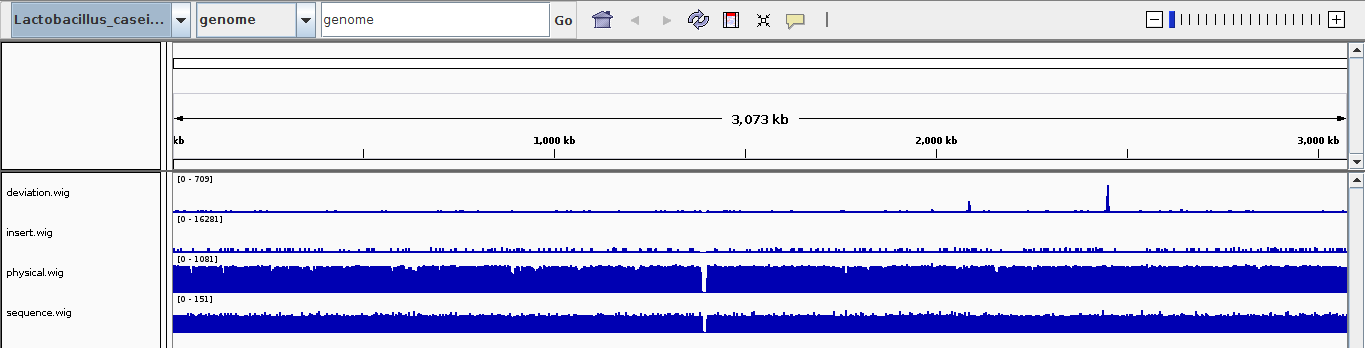
\includegraphics[scale=0.3]{tracks}
\caption{Tracks loaded on IGV}
\label{fig:tracks}
\end{figure}

In figure~\ref{fig:inserts} we could see a representation of the length of the
inserts. In the graph for each insert is displayed $insert\_length - mean$ and
the 2 lines represents respectively $standard\_deviation * 2$ (the orange one)
and $standard\_deviation * 3$ (the red one).
\begin{figure}[H]
\centering
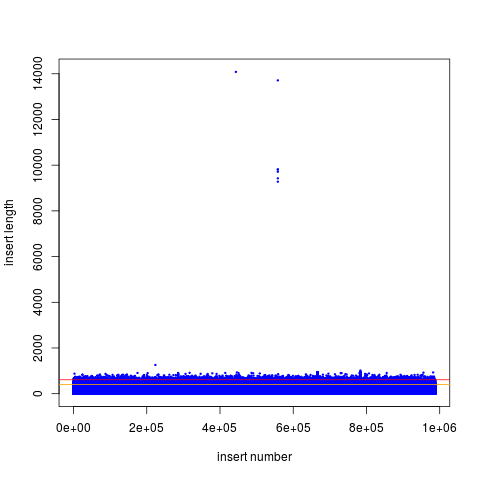
\includegraphics[scale=0.6]{inserts}
\caption{Inserts length graph}
\label{fig:inserts}
\end{figure}

In the graph~\ref{fig:inserts} we could see that some inserts are really long,
certain more than 12000 bases. The longest is 16281 bases long.

This graph is generated using R, using this script:
\lstinputlisting[language=R]{../code/plotinserts.R}
